% This is "sig-alternate.tex" V2.1 April 2013
% This file should be compiled with V2.5 of "sig-alternate.cls" May 2012
%
% This example file demonstrates the use of the 'sig-alternate.cls'
% V2.5 LaTeX2e document class file. It is for those submitting
% articles to ACM Conference Proceedings WHO DO NOT WISH TO
% STRICTLY ADHERE TO THE SIGS (PUBS-BOARD-ENDORSED) STYLE.
% The 'sig-alternate.cls' file will produce a similar-looking,
% albeit, 'tighter' paper resulting in, invariably, fewer pages.
%
% ----------------------------------------------------------------------------------------------------------------
% This .tex file (and associated .cls V2.5) produces:
%       1) The Permission Statement
%       2) The Conference (location) Info information
%       3) The Copyright Line with ACM data
%       4) NO page numbers
%
% as against the acm_proc_article-sp.cls file which
% DOES NOT produce 1) thru' 3) above.
%
% Using 'sig-alternate.cls' you have control, however, from within
% the source .tex file, over both the CopyrightYear
% (defaulted to 200X) and the ACM Copyright Data
% (defaulted to X-XXXXX-XX-X/XX/XX).
% e.g.
% \CopyrightYear{2007} will cause 2007 to appear in the copyright line.
% \crdata{0-12345-67-8/90/12} will cause 0-12345-67-8/90/12 to appear in the copyright line.
%
% ---------------------------------------------------------------------------------------------------------------
% This .tex source is an example which *does* use
% the .bib file (from which the .bbl file % is produced).
% REMEMBER HOWEVER: After having produced the .bbl file,
% and prior to final submission, you *NEED* to 'insert'
% your .bbl file into your source .tex file so as to provide
% ONE 'self-contained' source file.
%
% ================= IF YOU HAVE QUESTIONS =======================
% Questions regarding the SIGS styles, SIGS policies and
% procedures, Conferences etc. should be sent to
% Adrienne Griscti (griscti@acm.org)
%
% Technical questions _only_ to
% Gerald Murray (murray@hq.acm.org)
% ===============================================================
%
% For tracking purposes - this is V2.0 - May 2012

\documentclass{sig-alternate-05-2015}
\usepackage{hyperref}
\usepackage{float}

\begin{document}

% Copyright
\setcopyright{acmcopyright}
%\setcopyright{acmlicensed}
%\setcopyright{rightsretained}
%\setcopyright{usgov}
%\setcopyright{usgovmixed}
%\setcopyright{cagov}
%\setcopyright{cagovmixed}


% DOI
\doi{10.475/133_7}

% ISBN
\isbn{0000-42-1337}

%Conference
\conferenceinfo{Life '16}{May 25, 2016, DK}

\acmPrice{\$15.00}

%
% --- Author Metadata here ---
\conferenceinfo{DIKU}{'16 El Diku, Copenhagen}




\title{Secure E-mail}
\subtitle{[Ugeopgave 3]
\titlenote{}}
%
% You need the command \numberofauthors to handle the 'placement
% and alignment' of the authors beneath the title.
%
% For aesthetic reasons, we recommend 'three authors at a time'
% i.e. three 'name/affiliation blocks' be placed beneath the title.
%
% NOTE: You are NOT restricted in how many 'rows' of
% "name/affiliations" may appear. We just ask that you restrict
% the number of 'columns' to three.
%
% Because of the available 'opening page real-estate'
% we ask you to refrain from putting more than six authors
% (two rows with three columns) beneath the article title.
% More than six makes the first-page appear very cluttered indeed.
%
% Use the \alignauthor commands to handle the names
% and affiliations for an 'aesthetic maximum' of six authors.
% Add names, affiliations, addresses for
% the seventh etc. author(s) as the argument for the
% \additionalauthors command.
% These 'additional authors' will be output/set for you
% without further effort on your part as the last section in
% the body of your article BEFORE References or any Appendices.

\numberofauthors{1} %  in this sample file, there are a *total*
% of EIGHT authors. SIX appear on the 'first-page' (for formatting
% reasons) and the remaining two appear in the \additionalauthors section.
%
\author{
% You can go ahead and credit any number of authors here,
% e.g. one 'row of three' or two rows (consisting of one row of three
% and a second row of one, two or three).
%
% The command \alignauthor (no curly braces needed) should
% precede each author name, affiliation/snail-mail address and
% e-mail address. Additionally, tag each line of
% affiliation/address with \affaddr, and tag the
% e-mail address with \email.
%
% 1st. author
\alignauthor
Mirza Hasanbasic
}
% There's nothing stopping you putting the seventh, eighth, etc.
% author on the opening page (as the 'third row') but we ask,
% for aesthetic reasons that you place these 'additional authors'
% in the \additional authors block, viz.

% Just remember to make sure that the TOTAL number of authors
% is the number that will appear on the first page PLUS the
% number that will appear in the \additionalauthors section.

\maketitle
\begin{abstract}
In this assignment we are looking at how to create a secure way to send e-mails using PGP and thunderbird's plugin enigmail. Furthermore why the size of the key was chosen and why it could be a problem to upload the revocation to someone. Read till the end to see if it is safe to use this method as a way to safekeep it for passwords
\end{abstract}


%
% The code below should be generated by the tool at
% http://dl.acm.org/ccs.cfm
% Please copy and paste the code instead of the example below.
%
\begin{CCSXML}
<ccs2012>
 <concept>
  <concept_id>10010520.10010553.10010562</concept_id>
  <concept_desc>Computer systems organization~Embedded systems</concept_desc>
  <concept_significance>500</concept_significance>
 </concept>
 <concept>
  <concept_id>10010520.10010575.10010755</concept_id>
  <concept_desc>Computer systems organization~Redundancy</concept_desc>
  <concept_significance>300</concept_significance>
 </concept>
 <concept>
  <concept_id>10010520.10010553.10010554</concept_id>
  <concept_desc>Computer systems organization~Robotics</concept_desc>
  <concept_significance>100</concept_significance>
 </concept>
 <concept>
  <concept_id>10003033.10003083.10003095</concept_id>
  <concept_desc>Networks~Network reliability</concept_desc>
  <concept_significance>100</concept_significance>
 </concept>
</ccs2012>
\end{CCSXML}

\ccsdesc[500]{Computer systems organization~Embedded systems}
\ccsdesc[300]{Computer systems organization~Redundancy}
\ccsdesc{Computer systems organization~Robotics}
\ccsdesc[100]{Networks~Network reliability}


%
% End generated code
%

%
%  Use this command to print the description
%


% We no longer use \terms command
%\terms{Theory}

\section{Approach to the assignment}

The way I approached the assignment was to carefully read what I have to do. Hereafter I downloaded and installed thunderbird. When I was done installing thunderbird I found the enigmail plugin. But I had a problem installing PGP so I manually found PGP4WIN and installed this too. After this I created my key and uploaded it to pgp.mit.edu by copy the key to clipboard and upload it.

I have sent mails to \href{janro.datanet@gmail.com}{janro.datanet@gmail.com} and got it signed. More info in the appendix

\section{Choice of key}

I choose the key type RSA and the key size is 4096 because there were some weaknesses discovered in SHA-1, which is the hash used by DSA. The reason to go with the key size of 4096 is if by any chance someone managed to find a way to crack something of the size of 2048 in 100 hours, then this doesn't mean that it will take 200 hours to crack the 4096. The downside with using a key size of 4096 is that it uses more CPU and more storage space, but this should not be that big of a problem for the sake of security

Although both algorithms are based on mathematical problems which are not proven to be secure, then I cannot be more secure by using one over the other, but since DSA is using SHA-1 then I might have a bigger security problem than with RSA.

.
\section{Revocation}

If I upload the revocation certificate as part of the assignment, then anybody with access to it will be able to revoke my key and I will lose all of my reputation on the OpenPGP. This is the only consequence, they will not be able to gain access to my private key.
Since I probably never will need it unless my password gets stolen at any time then it will be a good idea to have the revocation certificate at hand at all time. This can be solved by creating a QR-code and print it. Hereafter I can delete the digital file and the only one who can access the revocation would be me with the QR-code.

\section{Safekeeping password}

The biggest problem can be some sort of compromise of the system. If I choose to store my key encrypted under a strong passphrase, then this could be compared to have the same risk as with a password manager. But if someone roots my system and manage to unlock my key then they will have all of my passwords. But since Eric is using his G-mail account, then it all depends on the Google teams ability to maintain security. It would still be a good idea to have a strong passphrase. This way it works kinda like double security. Someone would need both the G-mail password and the passphrase for the gpg key

But in the end the most important thing to remember is to have a strong passphrase, that contains both capitalization, numbers and special characters and this passphrase should be unique.

\newpage
\onecolumn
%APPENDICES are optional
%\balancecolumns
\appendix
%Appendix A
\section{Printout from MIT Key Server}
\begin{figure}[H]
  \centering
  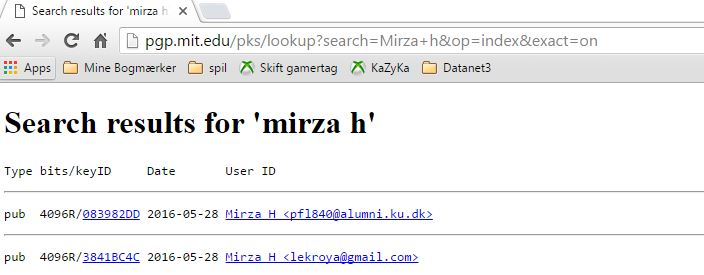
\includegraphics[scale=1]{MITKEY.jpg}
  \caption{Both my ku-mail and my personal mail}
\end{figure}
\newpage
\section{Email to TA}
\begin{figure}[H]
  \centering
  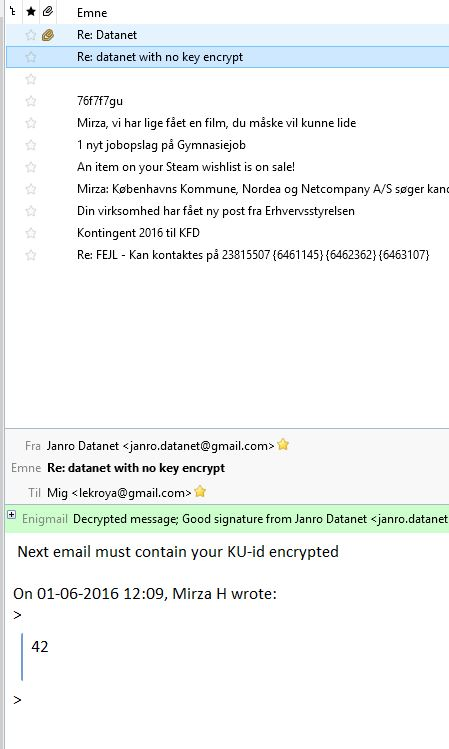
\includegraphics[scale=1]{ft.jpg}
  \caption{Showing that I sent an e-mail to a TA with the number 42}
\end{figure}
\begin{figure}[H]
  \centering
  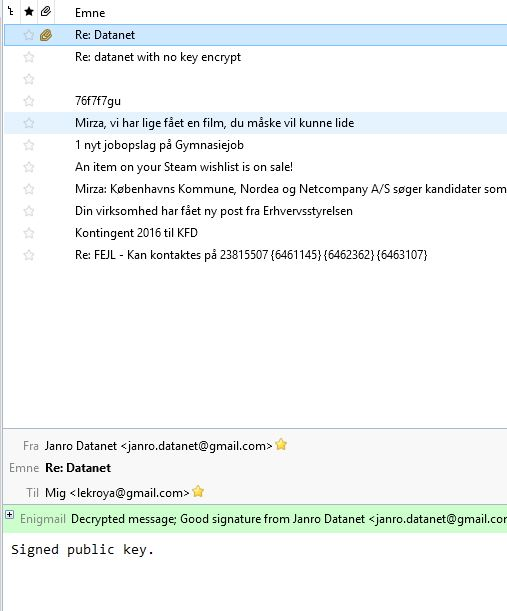
\includegraphics[scale=1]{signedkey.jpg}
  \caption{Showing that the TA signed the key}
\end{figure}
\begin{figure}[H]
  \centering
  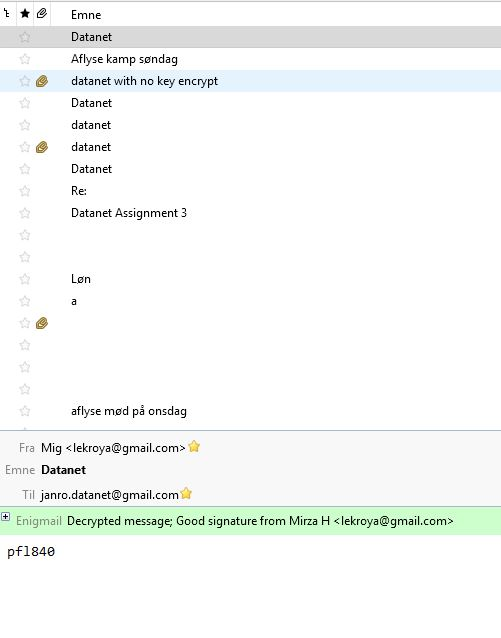
\includegraphics[scale=1]{pfl840.jpg}
  \caption{Showing that I sent an e-mail to a TA with my KU id}
\end{figure}
\begin{figure}[H]
  \centering
  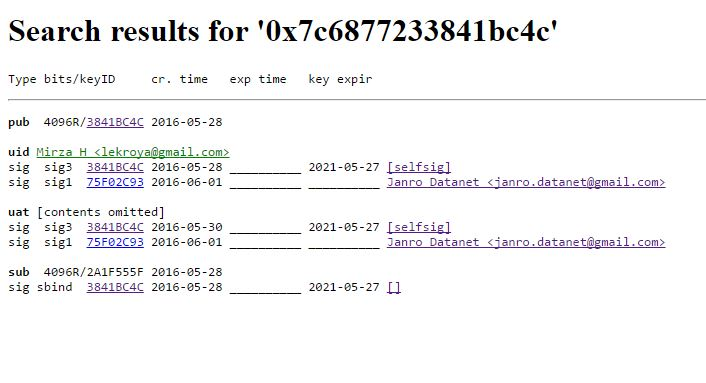
\includegraphics[scale=1]{mitsignedkey.jpg}
  \caption{Showing that the key has been signed}
\end{figure}






%\balancecolumns % GM June 2007
% That's all folks!
\end{document}
